Notes mostly based on \citet{maico2020categoria},
\citet{bradley2020topology}, \citet{borceux1994handbook}.
Whenever $\circledast$ is present, this indicates an original idea from the author,
thus, it should be taken with a grain of salt.

\section*{Notation}

Here is a small guideline on the notation used.

We usually refer to generic categories as $\mathcal C$ and similar uppercase letters with
curly font. For named categories (e.g. category of graphs, category of small categories,...)
we usually use a bold font with no italic, e.g. $\mathbf{Gr}, \mathbf{SmCat}, \mathbf{Top}$...

\begin{enumerate}
  \item $\circ$ - Used to symbolize composition of morphisms similar to how we compose functions.
  \item $\fatsemi$ - Represents composition, but with orders reversed, i.e. $g\circ f = f \fatsemi g$.
  \item $\diamond$ - \textit{Whiskering, prewhiskering, postwhiskering}.
  \item $\cong$ - Isomorphism in the context applied (e.g. categorical, set theoretical, etc).
  \item $\simeq$ - Equivalence of categories via natural transformations (weaker than isomorphism).
\end{enumerate}

\newpage
\section{Preface}

The study of Category Theory enables us to view Mathematics from a vantage
point, and better understand how the different areas are connected.
By looking at the subject from the distance (via Category Theory), we get
a glimpse at the connections (and disconnections) between different fields.

Another interesting observation about Category Theory is that it's
breaking the theoretical barrier and it's starting to be applied
in real world applications. One prominent example is in programming,
as highlighted by the book \citet{milewski2018category}.
The book by \citet{fong2019invitation} also focus on the application
side of Category Theory.

For those interested in applying Category Theory, Julia has a very
prominent package called Catlab.jl, which will be shown in these notes.

These notes are intended to serve as a quick introduction to people interested
in applying Category Theory. Thus, instead of focusing on proving theorems
or presenting a plethora of examples in mathematics, the goal is to rigorously
(and quickly) introduce the field together with some intuition and useful examples.

The notes start by introducing the \textbf{big 5} of Category Theory:
categories, functors, natural transformations, limits/colimits and adjoints.
After that, we focus on some applications of Category Theory,
mainly it's application to data structures/databases.

\newpage
\section{Categories}

In this section, we formally define what a category is, and we provide
some examples.

\subsection{Universes, Sets and Classes}

When working on Category Theory, it's common to find universal
statements such as ``for all topological spaces...''. The issue
with such statements is that, in a purely set-theoretical sense,
we have to know whether such large collection (``all topological spaces'')
is indeed a set. We might be tempted to say that's true, but
it's not so simple. The most known example of a possible failure of such
which the answer is ``no''.

statements is Russel's Paradox of whether there is a set of all sets, for
Therefore, in order to deal with such issue, we need a way to differentiate
between a valid set and an arbitrary collection. Here is where the notion of a Universe comes in.

\begin{definition}[Universe]
  We say that a set $\mathfrak U$ is a universe if\footnote{Definition from \citet{borceux1994handbook}}
  \begin{enumerate}[(i)]
    \item $x\in y$ and $ y\in \mathfrak U$, then $x \in \mathfrak U$;
    \item $I \in \mathfrak U$, and $\forall i \in I, x_i \in \mathfrak U$, then $\cup_{i\in I}x_i \in \mathfrak U$;
    \item $x \in \mathfrak U$ then $\mathcal P(x) \in \mathfrak U$, where $\mathcal P(x)$ is the power set;
    \item $x \in \mathfrak U$ and $f:x\to y$ is a surjective function, then $y \in \mathfrak U$;
    \item $\mathbb N \in \mathfrak U$.
  \end{enumerate}
\end{definition}

From this definition, one can prove the following proposition.
\begin{proposition}
  \begin{enumerate}[(i)]
    \item $x \in \mathfrak U$ and $y \subset x$, then $y \in \mathfrak U$;
    \item $x \in \mathfrak U$ and $y \subset x$, then $\{x,y\} \in \mathfrak U$;
    \item $x \in \mathfrak U$ and $y \subset x$, then $x\times y \in \mathfrak U$;
    \item $x \in \mathfrak U$ and $y \subset x$, then $y^x \in \mathfrak U$, where $y^x$ is the set of functions $f:x \to y$.
  \end{enumerate}
  \label{prop:universe}
\end{proposition}

With this definition, we state the axiom of existence universes.
\begin{axiom}
  Every set $S$ belongs to some universe $\mathfrak U$.
\end{axiom}

\begin{definition}
  For a fixed universe $\mathfrak U$, if a set $S$ is an element of $\mathfrak U$,
  then $S$ is called a \textit{small set}.
\end{definition}

Talking about ``small sets'' and ``big set'' might become daunting, so instead, we
use a different convention which is based on Gödel-Bernays theory of sets and classes.
This theory states that:
\begin{axiom}[Gödel-Bernays]
  Every set is a class, and a class is a set if and only if it belongs to some (other)
  class.
  \label{axiom:gb}
\end{axiom}

Note that using the notion of Universes, we can recover Gödel-Bernays theory. For that,
use the following definition:
\begin{definition}
  For a fixed universe $\mathfrak U$, we call $S$ a \textit{set} if it's an element
  of $\mathfrak U$, and call $S$ a \textit{class} if it's a subset of $\mathfrak U$.
  A class that is not a set is called a \textit{proper class}.
\end{definition}
Since every set is a class, if $S \in \mathfrak U$, then $S$ is a class,
since $U$ is a set and therefore a class, implying that $S$ belongs to a class.
On the other direction, if $S$ is a class and $S \in V \subset \mathfrak U$,
then since $V \subset \mathfrak U$, this means that $S \in \mathfrak U$, thus
it's a set.

From now on, whenever we say \textit{set} we are implying \textit{small set}
and whenever we say \textit{class} we are implying either small or big sets,
following \citet{borceux1994handbook} convention.


\subsection{What is a Category?}

Let's formally define a category and provide some examples.

\begin{definition}[Category]
	A category $\mathcal C = \langle Ob_{\mathcal C}, Mor_{\mathcal C} \rangle$ consists
	of a class of objects $Ob_\mathcal C$ and a class of morphisms
	$Mor_\mathcal C$ satisfying the following conditions:
  \begin{enumerate}[(i)]
    \item Every morphism $f \in Mor_\mathcal C$ is associated to two objects $X,Y \in Ob_{\mathcal C}$
      which is represented by $f:X \to Y$ or $X \xrightarrow{\hspace{3mm}f \hspace{3mm}} Y$,
      where $dom(f) = X$ is called the domain of $f$ and $cod(f)=Y$ is the codomain. Moreover, we define
      $Mor_\mathcal C (X,Y)$ as 
      \begin{displaymath}
        Mor_\mathcal C (X,Y) := \{f \in Mor_\mathcal C \ : \ X \in dom(f), \ Y \in cod(f)\};
      \end{displaymath}
    \item For any three objects $X,Y, Z \in Ob_\mathcal C$, there exists a composition operator
      \begin{displaymath}
        \circ: Mor_\mathcal C (X,Y)   \times Mor_\mathcal C (Y,Z) \to Mor_\mathcal C (X,Z),
      \end{displaymath}
      \item For each object $X \in Ob_\mathcal C$ there exists a morfism $id_X \in Mor_\mathcal C (A,A)$
        called the identity.
  \end{enumerate}
  The composition operator must have the following properties:
  \begin{enumerate}[(p.1)]
    \item \textit{Associative}: for every $f \in Mor_\mathcal C (A,B),
      g \in Mor_\mathcal C (B,C), h \in Mor_\mathcal C (C,D)$ then
      \begin{displaymath}
        h \circ (g \circ f) = (h \circ g) \circ f.
      \end{displaymath}
    \item For any $f \in Mor_\mathcal C (X,Y)$, $g \in Mor_\mathcal C (Y,X)$, 
      \begin{displaymath}
        f \circ id_X = f,  \quad id_Y \circ g = g.
      \end{displaymath}
  \end{enumerate}
\end{definition}

There are many ways to refers to the class of morphisms $Mor_\mathcal C (X,Y)$, such as
$\mathcal C(X,Y)$ or $\text{hom}_\mathcal C (X,Y)$. The reason for this is that
this set is sometimes called hom-set. In this notes, we'll use either $Mor_\mathcal C (X,Y)$
or $\mathcal C (X,Y)$ when there is no ambiguity. Also, we'll use $dom_f$ to mean $dom(f)$,
and similarly for the codomain.

Another point about conventions. When talking about composition, it's convenient
to use the operator $\fatsemi$, which is equivalent to the composition $\circ$,
but with the inverted order, i.e. $f \fatsemi g = g \circ f$. The convinience
will become clearer once we introduce Hasse diagrams as a way to represent categories.

When the class of morphism $Mor_\mathcal C(A,B)$ for every pair or objects is a set,
the category $\mathcal C$ is called a \textit{locally small category}\footnote{Note
that $Mor_\mathcal C$ can be a class while each $Mor_\mathcal C(A,B)$ is a set}.
If both $Ob_\mathcal C$ and $Mor_\mathcal C$ are sets, we then have a \textit{small category}.

Finally, whenever it's not ambiguous, we might drop the subscript and use $Ob$
to refer to the objects of $\mathcal C$ and $Mor$ to refer to the morphisms of $\mathcal C$.

\subsection{Examples of Categories}

It's very common to represent categories via Hasse Diagrams. In these diagrams, the
objects are represented as dots, and the morphisms as arrows. Let's show some examples.

\begin{example}[Category $\bm 1$]
  The category $\bm 1$ consists of $Ob_{\bm 1} := \{A\}$ and $Mor_{\bm 1} = \{id_A\}$.
  The diagram for such category is shown below.
  \begin{figure}[H]
    \begin{center}
      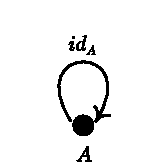
\includegraphics{./notebooks/1Cat}
    \end{center}
    \caption{Hasse diagram of category $\bm 1$.}
    \label{fig:1Cat}
  \end{figure}
\end{example}

\begin{example}[Category $\bm 2$ and $\bm 3$]
  The category $\bm 2$ consists of $Ob_{\bm 2} := \{A, B\}$ and $Mor_{\bm 1} = \{id_A, id_B, f\}$,
  where $f:A \to B$.
  The diagram for such category is shown below.
  \begin{figure}[H]
    \begin{center}
      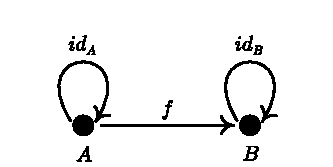
\includegraphics{./notebooks/2Cat}
    \end{center}
    \caption{Hasse diagram of category $\bm 2$.}
    \label{fig:2Cat}
  \end{figure}

Since we know that identities are always present in categories, we'll
omit them from future diagrams when there is no ambiguity. Thus,
the figure below represents the same diagram as Figure \ref{fig:2Cat}.
\begin{figure}[H]
  \begin{center}
    
\includegraphics{./notebooks/2Catsimple}
  \end{center}
  \caption{Hasse diagram of category $\bm 2$ omitting identity morphisms.}
  \label{fig:2Catsimple}
\end{figure}

The category $\bm 3$ has three morphisms besides the identities, given
by $f$, $g$ and their composition $f \fatsemi g$. The figure below
illustrates the category with all it's morphisms.

\begin{figure}[H]
  \begin{center}
    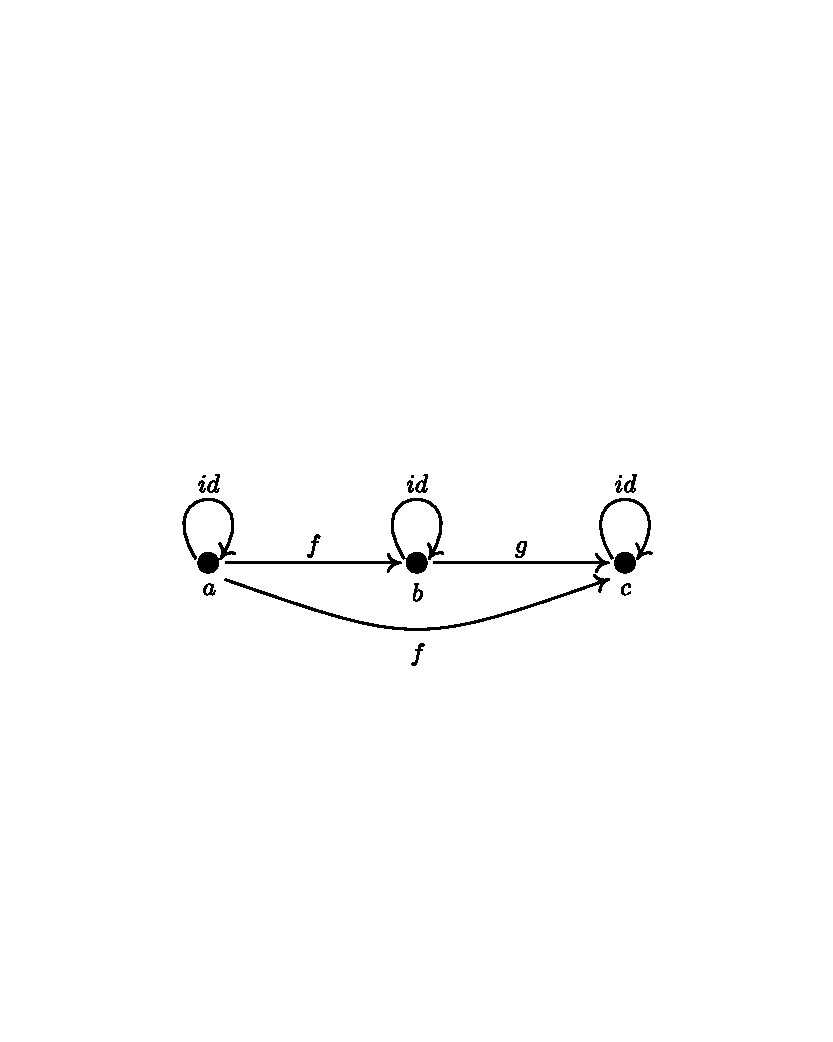
\includegraphics{./notebooks/3CatComplete}
  \end{center}
  \caption{Hasse diagram of category $\bm 3$ showing all morphisms.}
  \label{fig:3Catcomplete}
\end{figure}

Drawing all the morphisms can make the diagram become too crowded, specially
as the number of objects and morphisms grows. Hence, we simplify the
diagram representation by ommiting not only the identity morphisms, but also
the compositions. These can always be assumed to exist, since they are a necessery
condition for every category.
Thus, the figure below represents the same diagram as Figure \ref{fig:3Catcomplete}.

\begin{figure}[H]
  \begin{center}
    
\includegraphics{./notebooks/3Catsimple}
  \end{center}
  \caption{Hasse diagram of category $\bm 3$ omitting identities and compositions.}
  \label{fig:3Catsimple}
\end{figure}

\end{example}

\begin{example}[Discrete Categories]
  The discrete category $\mathbf{\underline{N}}$ is the category with $N$ objects
  and $Mor_{\mathbf{\underline{N}}} := \{id_1,...,id_N\}$. An example of this category is
  illustrated below.

  \begin{figure}[H]
    \begin{center}
      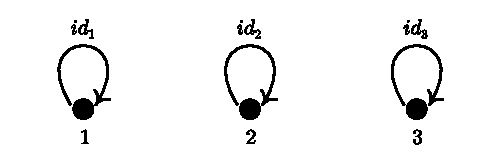
\includegraphics{./notebooks/3Discrete.pdf}
    \end{center}
    \caption{Example of category $\mathbf{\underline{3}}$.}
    \label{fig:3Discrete}
  \end{figure}
\end{example}

\begin{example}[Preorders]
  A preorder is defined by a tuple $(P, \leq)$, where $P$ is a set of values, such that
  \begin{enumerate}[(i)]
    \item For $a,b \in P$, if $a\leq b$ and $b \leq c$, then $a \leq c$;
    \item For every $a \in P$, $a \leq a$.
  \end{enumerate}
  We can show that actually, this is a category, which we'll call $\mathcal P$,
  where $Ob_\mathcal P = P$ and each morphism $f$ represents $a \leq b$, where
  $cod_f = a$ and $dom_f = b$.
  One example of preorder is the set of $\mathbb N$ equiped with the binary relation $\leq$
  which is shown in the diagram below.

\begin{figure}[H]
  \begin{center}
    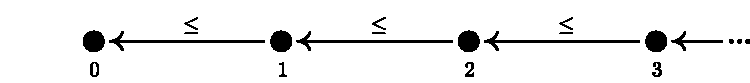
\includegraphics{./notebooks/NCat}
  \end{center}
  \caption{Hasse diagram of preorder category of natural numbers.}
  \label{fig:NCat}
\end{figure}
\end{example}

Note that in preorders, there is at most one morphism between each pair of objects.
Thus, categories with such property are often referred as \textit{thin categories}
or \textit{preorder category} (in \citet{fong2019invitation}, the authors call this
a \textit{preorder reflection}).

\begin{example}[Monoids]
  A monoid is a triple $(M, \oplus, e_M)$ where $\oplus:M\times M \to M$ is a binary operation
  and $e_M$ the neutral element, such that:
  \begin{enumerate}
    \item $a \oplus (b \oplus c) = (a \oplus b) \oplus c$
    \item $a \oplus e_M = e_M \oplus a = a$.
  \end{enumerate}
  Note that $(\mathbb N \cup\{ 0\}, +, 0)$ is a monoid.

  Moreover, each single monoid can be defined as a category itself. For
  monoid $(M, \oplus, e_M)$, define a category $\mathcal C$
  such that $Ob_\mathcal C := \{M\}$, and the set of morphisms
  are the elements of $M$, i.e.
  $Mor_\mathcal C := \{a \in M\}$. Finally, we define the composition
  operartion as $a \circ b := a \oplus b$
  Thus, $(\mathbb N \cup \{0\}, +, 0)$ is the category illustrated in
  Figure \ref{fig:NMonoid}.

  \begin{figure}[H]
    \begin{center}
      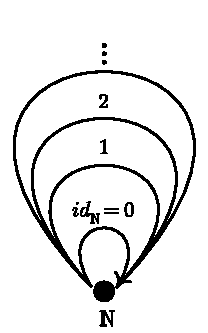
\includegraphics{./notebooks/NMonoid}
    \end{center}
    \caption{Hasse diagram of monoid category of natural numbers.}
    \label{fig:NMonoid}
  \end{figure}
  
\end{example}

There are many other examples:
\begin{enumerate}[1.]
  \item $\mathbf{Set}$ which is the category of sets, where the objects are sets and the morphisms are functions between sets.
  \item $\mathbf{Top}$ is the category where topological spaces are the objects and continuous functions are the morphisms.
  \item $\mathbf{Vec}_\mathbb F$ is the category where vector spaces over field $\mathbb F$ are the objects,
    and linear transformations are the morphisms.
  \item $\mathbf{Gr}$ is the category of directed graphs, where $Ob_{\mathbf{Gr}} := \{\text{Vertex}, \text{Arrow}\}$,
    and the morphisms are
    \begin{displaymath}
      Mor_{\mathbf{Gr}} := \{
        src,
        tgt,
        id_{\text{Vertex}},
        id_{\text{Arrow}}
      \}
    \end{displaymath}
    where $src:\text{Arrow} \to \text{Vertex}$ returns the source vertex for each arrow and
    $tgt:\text{Arrow} \to \text{Vertex}$ returns the target vertex.
\end{enumerate}


\subsection{Programming with Category Theory}

One might be surprised to find out that Category Theory,
although very abstract in nature, has actual applications in the
``real world''. A very interesting example of this is in programming.

In programming languages such as Julia, we can think of `Types`
as objects and functions as morphisms.

\subsection{Isomorphism, monomorphism and epimorphism}

A very important definition in Category Theory is the notion of isomorphism.
In Set Theory, we say that two sets are isomorphic if there is an invertible
function between them. Yet, this concept is not restricted to Set Theory
and can be generalized in Category Theory as follows:

\begin{definition}[Categorical Isomorphism]
  Let $\mathcal C$ be a category with $X,Y \in Ob_\mathcal C$ and $f \in Mor_\mathcal C (X,Y)$.
  \begin{enumerate}[(i)]
    \item We say that $f$ is \textit{left invertible} if there exists $f_l \in Mor_\mathcal C (Y,X)$ such
      that $f_l \circ f = id_X$;
    \item We say that $f$ is \textit{right invertible} if there exists $f_r \in Mor_\mathcal C (Y,X)$ such
      that $f \circ f_r = id_Y$;
    \item We say that $f$ is invertible if it's both left and right invertible.
  \end{enumerate}
  When an invertible morphism exists between $X$ and $Y$, we say that they are isomorphic.
  \label{def:CategoricalIsomorphism}
\end{definition}

\begin{proposition}
  The following properties on inverses are true:
  \begin{enumerate}[1.]
    \item If $f$ is an invertible morphism, then the left and right inverses are the same.
    \item If $f$ and $g$ are invertible and composable, then $f \circ g$ is also invertible.
  \end{enumerate}
\end{proposition}
\begin{proof}
1. Let $f$ be invertible with left inverse $f_l$ and right inverse $f_r$. Therefore,
\begin{displaymath}
  f_l \circ id_Y = f_l \circ f \circ f_r = id_X \circ f_r = f_r.
\end{displaymath}

2. Let $f:A\to B$ and $g: B \to C$ be invertible and composable, with $f\circ g: A \to C$.
There exists the inverses $g^{-1}: C \to B$ and $f^{-1}:B \to A$. Note that
$f^{-1}\circ g^{-1}:C \to A$, thus
\begin{align*}
  (f^{-1} \circ g^{-1}) \circ (g \circ f) =
  f^{-1} \circ (g^{-1} \circ g) \circ f =
  (f^{-1} \circ id_B) \circ f =
  f^{-1} \circ f =
  id_A.
\end{align*}
\begin{align*}
  (g \circ f) \circ (f^{-1} \circ g^{-1})  =
  g \circ (f \circ f^{-1}) \circ g^{-1} =
  g \circ (id_B \circ g^{-1}) =
  g \circ g^{-1} =
  id_B.
\end{align*}
We conclude that $(g\circ f)^{-1} = f^{-1} \circ g^{-1}$.
  
\end{proof}
Although similar to set isomorphism, categorical isomorphism is in a sense more general,
and captures our intuition of isomorphism between categories better than the set theoretic case,
even when we have finite objects.

Consider the following example.
Let $\mathcal P$ be the category of Posets, where posets $(P,\leq_p)$ are the objects.
Take two objects $P_1, P_2 \in Ob_\mathcal P$,
where $P_1:=\{a,b\}$ with $a$ and $b$ \textbf{not} comparable,
and $P_2:=\{0,1\}$ where indeed $0 \leq 1$. The question is whether $P_1$ is ``actually'' isomorphic
to $P_2$, and our intuition say that they should not be, since 
$P_1$ has two incomparable elements while $P_2$ has two comparable elements.

If we use the set theoretic definition, we would conclude that they \textbf{are} isomorphic,
since there is a bijective function between $P_1$ and $P_2$. 
Take for example $f:P_1\to P_2$ where $f(a)=0$ and $f(b)=1$.
So the set theoretic isomorphism does not capture what we want. What about the categorical isomorphism?
We can prove that this will not be an isomorphism using the categorical definition. Yet,
in order to prove this, we need to specify what are the morphisms between the posets,
and to do this, we need to define what are functors.

In the same way that set isomorphism is not the same as categorical isomorphism,
the notions of injectivity and surjectivity are not equivalent to their categorical
counterparts, which are called monomorphism and epimorphism.

\begin{definition}[Monomorphism]
  Let $\mathcal C$ be a category and $f \in Mor_\mathcal C(A,B)$. We say that
  $f$ is a monomorphism (or monic), if
  \begin{displaymath}
    f \circ g = f \circ h \implies g = h.  
  \end{displaymath}
\end{definition}

\begin{definition}[Epimorphism]
  Let $\mathcal C$ be a category and $f \in Mor_\mathcal C(A,B)$. We say that
  $f$ is an epimorphism (or epic), if
  \begin{displaymath}
    g \circ f = h \circ f \implies g = h.
  \end{displaymath}
\end{definition}
\textbf{Important!} A morphism $f$ can be both epic and monic, without being
an isomorphism, which again highlights the difference between this concepts and their
set-theoretic counterparts.

\begin{proposition}
  The following properties on monomorphism and epimorphism are true:
  \begin{enumerate}[1.]
    \item $f$ left-invertible $\implies$ $f$ is monic. The converse are is not true.
    \item $f$ right-invertible $\implies$ $f$ is epic. The converse are is not true.
    \item $f$ invertible $\implies$ $f$ is monic and epic. The converse are is not true.
    \item $f$ monic and right-invertible $\implies $ $f$ is isomorphism.
    \item $f$ epic and left-invertible $\implies $ $f$ is isomorphism.
  \end{enumerate}
\end{proposition}

\begin{proof}
1. Note $f:A \to B$ left-invertible implies that there exists a $f_l:B \to A$ such that
$f_l \circ f = id$. Hence, for a $g:B\to C$ and $h: B \to C$, if
\begin{displaymath}
  f \circ g = f \circ h,
\end{displaymath}
then we have that
\begin{displaymath}
  f_l \circ f \circ g = f_l \circ f \circ h \implies g =h.
\end{displaymath}
To show that the converse is false, consider the category $\mathbf{2}$(Figure \ref{fig:2Cat}). Note that
$f:A\to B$ is monic, since the only morphism that composes with $f$ is
$id_A$ and $id_B$. Yet, note that $f$ is not left invertible, since there isn't even
a morphism from $B$ to $A$.

2. Use the same argument, but reversing the order of the compositions.
For the converse, again consider the same category $\mathbf{2}$. Note that
$f:A\to B$ is epic, but it's not right invertible.

3. True since invertible means left and right invertible.

4. Since $f:A \to B$ right invertible, then there exists $f_r:B \to A$
such that $f \circ f_r = id_B$. Thus,
\begin{displaymath}
  id_B \circ f = (f \circ f_r) \circ f =
  f \circ (f_r \circ f) =
  f \circ id_A \implies f_r \circ f = id_A.
\end{displaymath}
5. Same argument.
\end{proof}

\subsection{Zero, Initial and Terminal Objects}

\begin{definition}[Zero, Initial and Terminal]
  Let $\mathcal C$ be a category.
  \begin{enumerate}[1.]
    \item An object $I \in Ob_\mathcal C$ is \textit{initial} if for every $A \in Ob_\mathcal C$,
      there is exactly one morphism from $I$ to $A$. Thus, from $I$ to $I$ there is only the identity.
    \item An object $T \in Ob_\mathcal C$ is \textit{terminal} if for every $A \in Ob_\mathcal C$,
      there is exactly one morphism from $A$ to $T$. Thus, from $I$ to $I$ there is only the identity.
    \item An object is \textit{zero} if it's both terminal and initial.
  \end{enumerate}
\end{definition}

Note that in the definitions above, we are defining these objects in terms of existence and
uniqueness of morphisms, which is known in category theory as \textbf{universal constructions}
(more on this later).

\begin{theorem}
  Every \textit{initial} object is unique up to an isomorphism, i.e. if in a category there 
  are two \textit{initial} objects, then they are isomorphic.
  Similarly, \textit{terminal} objects are unique up to an isomorphism.
  Moreover, the isomorphism is unique between initial object, and between terminal objects.
\end{theorem}
\begin{proof}
  Let $I_1, I_2$ be initial. Then, there exists only $f:I_1 \to I_2$ and $g:I_2 \to I_1$.
  But since $g \circ f:I_1 \to I_1$ is a morphism from the initial object $I_1$, it must
  be equal to $id_{I_1}$. The same for $I_2$, which implies that $f$ and $g$ are inverses,
  and thus the objects are isomorphic. Since both $f$ and $g$ are the only morphisms from
  $I_1$ and $I_2$, this also implies that their are the only isomorphism.
  The same proof works for terminal objects.
\end{proof}


\begin{example}[Terminal and Initial Objects in $\mathbf{Set}$]
Without thinking too much, one might assumet that in the category $\mathbf{Set}$
the empty set would be a zero object; but that's not true.
In reality, the empty set is the initial object, since $f:\varnothing \to B$
is the only function from the empty set to any other set. Why is this valid?

Remember that in set theory, a function from two sets is defined as a binary
relation such that for every $x \in dom_f$, there is a unique $y \in cod_f$, i.e.
$f$ is a triple $(A,B,G)$, where $A = dom_f$, $B = cod_f$ and $G \subset A \times B$
such that $\forall x \in dom_f$, there exists a unique $y \in B$, such that $(x,y) \in G$.

Since $dom_f = \varnothing$, we have that $G \subset \varnothing \times B$, but this
is actually empty. Why? If $\varnothing \times B$ is not empty, then there exists
$(a,b) \in \varnothing \times B$, which is false, since this would imply that
$a \in \varnothing$, which contradicts the definition of the empty set that says
that it can have no elements (note that $\varnothing \in \varnothing$ is actually false).

With this, we have that $G = \varnothing$, thus, the only possible function from
$\varnothing$ to $B$ is $f = (\varnothing, \varnothing, B)$. Which proves that the
empty set is initial.

But what about terminal? The empty set actually does not have any morphisms
that arrives on it, since there is no function $f:A \to \varnothing$.
The terminal sets in $\mathbf{Set}$ are actually all the singletons (sets with only
one element), since for any $\{a\}$, there will be only one function
$g: A \to \{a\}$, which is $g(x) = a$.
\label{ex:InitialTerminalSet}
\end{example}

Another definition we have is that of a \textit{zero} morphism. The idea here
is that this morphism must take the elements of an object $A$ to the
zero element in $B$, for example, a for two vector spaces $\mathbb R^n$ and $\mathbb R^m$,
the zero linear transformation $z:\mathbb R^n \to \mathbb R^m$ should take every vector
$n$-dimensional vector to the $\mathbf{0}$ $m$-dimensional vector. In Category
Theory we do not talk about morphisms according to how they act on the elements, but
only in the objects. So we cannot define $z$ by saying to which element it maps.
Yet, there is a way to do this in Category Theory, which gives rise to the \textit{zero} morphism
definition.
\begin{definition}[Zero Morphism]
  Let $\mathcal C$ be a category, and $0$ be a zero object.
  A morphism $z:A \to B$ is a zero morphism if there exists two morphisms
  $f:A\to 0$ and $g:0 \to B$, such that
  \begin{displaymath}
    z = g \circ f.  
  \end{displaymath}
\end{definition}
See that this makes intuitive sense. In our example, since we wish to take
$v \in \mathbb R^n$ to $0 \in \mathbb R^m$, we first take all $v$ to the zero object,
which in the category of vector spaces will be the zero vector space, i.e. $\{0\}$ the space
where $0 \in \mathbb R$ is the only element. So now all $v$ are $0$. Note that
every linear transformation from $\{0\}$ to $\mathbb R^m$ must take $0$ to $\mathbf{0} \in \mathbb R^m$,
otherwise, suppose that $g(0)=\mathbf{v} \neq \mathbf{0}$, hence for a scalar $\alpha$,
\begin{displaymath}
  g(0) = g(\alpha0) = \mathbf{v} \neq \alpha \mathbf{v} = \alpha g(0).
\end{displaymath}
This is a contradiction, since $g$ is a linear transformation.

\begin{theorem}
  Let $\mathcal C$ be a catgory with zero object $0$.
  Then there exists a unique zero morphism between any two objects.
\end{theorem}
\begin{proof}
  Let $A, B \in Ob_\mathcal C$.
  By the definition of the zero object, there exists a unique 
  $f:A \to 0$ and $g:0\to B$, thus, $g \circ f$ is a zero morphism
  by definition and is unique, since there is no other $f$ and $g$ with these respective
  domain and codamain.

  Moreover, note that if $z:A \to B$ is our zero morphism and $h:B \to C$, then
  \begin{displaymath}
    h \circ z = h \circ (g \circ f) = (h \circ g) \circ f.
  \end{displaymath}
  But, $l =(h \circ g):0 \to C$, which means that $l \circ f$ is a zero morphism.
  The same argument works with a composition from the other direction. This means
  that compositions with zero morphisms return zero morphisms.
\end{proof}

\subsection{Understanding Duality}

In several fields of Mathematics, one is faced with the informal notion of a dual.
Mathematicians define a concept, and call them the dual in some sense, for example,
the dual vector space, the dual of an optimization problem, and many more.
I always found puzzling what exactly held these things together, i.e.
what was the underlying principle that made something a dual of another.

Fortunately, Category Theory has a very elegant answer. For a given
category $\mathcal C$, the dual category is denoted by
$\mathcal C^{op}$ where are the objects are the same, but the morphisms
are inverted. This means that $Ob_{\mathcal C} = Ob_{\mathcal C^{op}}$,
and for every $f\in Mor_\mathcal (A,B)$, we have $f^{op} \in Mor_{\mathcal C^{op}}(B,A)$.

This definition gives rise to a very interesting result (observation), called the
\textit{Duality Principle}.

\begin{definition}[Dual Property and Dual Statement]
  We say $p^{op}$ is the dual property for $p$ if for all categories
  \begin{displaymath}
    \mathcal C \text{ has }p^{op} \iff
    \mathcal C^{op} \text{ has }p.
  \end{displaymath}

  For a statement $s$ about a category $\mathcal C$, the dual statement is the same
  statement, but with regards to $\mathcal C^{op}$.
  \label{def:DualProperty}
\end{definition}
For example, ``a category has an initial object if and only if the dual category has a terminal object''.
In this example, the property of having an initial object is the dual property of having a terminal object,
since the above statement is true for any category.
What about the dual statement? The dual for the statement ``the category $\mathcal C$ has an initial object''
is ``the category $\mathcal C^{op}$ has an initial object''. Note that the dual statement is not always true.
And here is where we get the duality principle.

\begin{definition}[Duality Principle]
  If a statement $s$ is true for every category, then the dual statement is also true for every
  category.
\end{definition}
Let's digest a bit what this principle states. If we can prove that a certain statement is
true for any arbitrary category, then it's dual will also be true without any effort what so ever.
\citet{roman2017introduction} gives a nice example of this. We already prove that for any
category, if an initial object exists, this initial object is unique up to an isomorphism.
Note that this is a statement that is true for any category, so the duality principle applies,
i.e. the dual statement is true. And what is the dual statement? That for every $\mathcal C^{op}$
the initial object is unique up to an isomorphism. But an initial object in $\mathcal C^{op}$
is a terminal object in $\mathcal C$. So we have, without any effort, that every terminal
object is unique up to an isomorphism.

\subsection{Categorical Product and Coproduct}

In set theory, we are used to the notion of a Cartesian product. Similarly
to how we did for isomorphism, the idea of a product can be generalized via
Category Theory. Here is how it's done.

\begin{definition}[Span]
  Let $A,B$ be objects in a  category $\mathcal C$. A span
  on $A$ and $B$ is a triple $(Z,f,g)$ where $f:Z\to A$ and
  $g:Z\to B$ are morphisms in $\mathcal C$. This is
  shown in figure \ref{fig:Span}.
  \label{def:Span}
\end{definition}

\begin{figure}[H]
  \begin{center}
    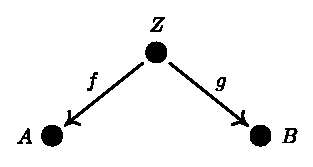
\includegraphics{./notebooks/Span.pdf}
  \end{center}
  \caption{Diagrams showcasing a span between $A$ and $B$.}
  \label{fig:Span}
\end{figure}

\begin{definition}[Categorical Product]
  Let $A,B$ be objects in a  category $\mathcal C$. A span $(A\times B, \pi_1, \pi_2)$
  is called a product between $A$ and $B$ if for every span $(Z, f, g)$ of $A$ and $B$,
  there exists a unique morphism $h_{f,g}:Z \to A \times B$ such that
  $h_{f,g} \fatsemi \pi_1 = f$ and $h_{f,g} \fatsemi \pi_2 = g$. That is the same
  as saying that the diagram \ref{fig:Product} commutes.
\end{definition}

\begin{figure}[H]
  \begin{center}
    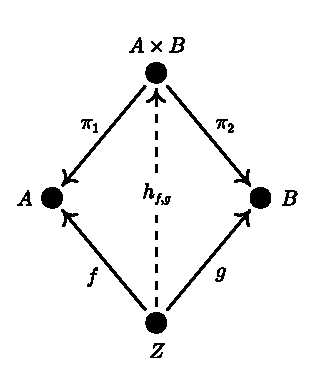
\includegraphics{./notebooks/CategoricalProduct.pdf}
  \end{center}
  \caption{Diagrams showcasing the categorical product. Note that the dashed line
  is intended to highlight that the morphism $h_{f,g}$ is uniquely induced by $f$ and $g$.}
  \label{fig:Product}
\end{figure}

Note that this definition of a product is a \textbf{universal construction}, since
it's done via existence and uniqueness.
Another important aspect to note is that not every pair of objects in a category might have a
product associated.

\begin{theorem}
  For a category $\mathcal C$, a pair of objects $A$ and $B$ can have more than one
  product construction, but if this is the case, then both these constructions will be
  isomorphic.
\end{theorem}

\begin{proposition}[Categorical Product vs Set Product]
  The categorical product generalizes the Cartesian product in set theory.
\end{proposition}
\begin{proof}
  Consider the span $(X\times Y, \pi_1,\pi_2)$ where $\pi_1(x,y) = x$ and $\pi_2(x,y) = y$.
  Thus, for any span $(Z, f, g)$ of $A$ and $B$, make $h_{f,g}(z) = (f(z), g(z)) \in X \times Y$.
  This is how the Cartesian product works.

  Let's drop the subscript in $h_{f,g}$.
  Now we have to show that $h$ is a unique morphism,
  and that $h \fatsemi \pi_1 = f$ and $h \fatsemi \pi_2 = g$.

  The second condition is trivially true, just note that
  \begin{displaymath}
    \forall z \in Z, \ \pi_1(h(z)) = \pi_1((f(z), g(z))) = f(z) \implies
    h \fatsemi \pi_1 = f,
  \end{displaymath}
  and the same argument works for $\pi_2$ and $g$.

  For uniqueness, consider $h':Z\to X\times Y$ such that
  $h' \fatsemi \pi_1 = f$, and $h' \fatsemi \pi_2 = g$.
  If $h' \neq h$, then there is a $z \in Z$,
  such that $h(z) = (f(z), g(z)) \neq h'(z)$. Bu then,
  $\pi_1(h'(z)) \neq f(z)$ or $\pi_2(h'(z)) \neq g(z)$, which
  is a contradiction.

\end{proof}

From the definition of a product, it's easy to think of possible dual constructions
by just inverting the arrows (morphisms).

\begin{definition}[Cospan]
  Let $A,B$ be objects in a  category $\mathcal C$. A cospan
  on $A$ and $B$ is a triple $(Z,f,g)$ where $f:A\to Z$ and
  $g:B\to Z$ are morphisms in $\mathcal C$. This is
  shown in Figure \ref{fig:Cospan}.
\end{definition}

\begin{figure}[H]
  \begin{center}
    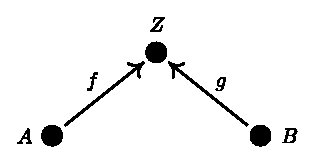
\includegraphics{./notebooks/Cospan.pdf}
  \end{center}
  \caption{Diagrams showcasing a cospan between $A$ and $B$.}
  \label{fig:Cospan}
\end{figure}

\begin{definition}[Categorical Coproduct]
  Let $A,B$ be objects in a  category $\mathcal C$. A cospan $(A + B, i_1, i_2)$
  is called a product between $A$ and $B$ if for every span $(Z, f, g)$ of $A$ and $B$,
  there exists a unique morphism $h_{f,g}:Z \to A \times B$ such that
  $i_1 \fatsemi h_{f,g} = f$ and $i_2 \fatsemi h_{f,g} = g$. That is the same
  as saying that the diagram \ref{fig:Coproduct} commutes.
\end{definition}

\begin{figure}[H]
  \begin{center}
    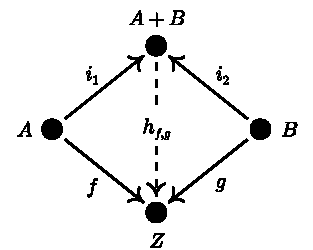
\includegraphics{./notebooks/CategoricalCoproduct.pdf}
  \end{center}
  \caption{Diagrams showcasing the categorical coproduct. Note that the dashed line
  is intended to highlight that the morphism $h_{f,g}$ is uniquely induced by $f$ and $g$.}
  \label{fig:Coproduct}
\end{figure}

While the categorical product was constructed to generalize the Cartesian set product,
the coproduct was constructed in Category Theory, so the question is
``to what does the coproduct corresponds in set theory?''. The answer is the
disjoint union! It's not a coincidence that we used ``$+$'' to symbolize it.

The idea of a product construction induced the notion of a product object
$A \times B$. Yet, this construction also induces another definition, of the
so called (co)product morphism.

\begin{definition}[Product and Coproduct Morphism]
  Let $A, B, C, D \in Ob_\mathcal C$,
  $(A\times B, \pi^{A,B}_1, \pi^{A,B}_2)$ and
  $(C\times D, \pi^{C,D}_1, \pi^{C,D}_2)$ two products in the category $\mathcal C$,
  $f:A\to C$ and $g:B \to D$ two morphisms in $\mathcal C$. Hence, the
  morphism induced by $\pi_1^{A,B} \fatsemi f$ and $\pi_2^{A,B} \fatsemi g$ is
  called product morphism and denoted by $f \times g$, where
  \begin{displaymath}
    f \times g := (\pi_1^{A,B} \fatsemi f, \pi_2^{A,B} \fatsemi g): A\times B \to C \times D.
  \end{displaymath}
\end{definition}

\begin{theorem}
  The product morphism $f\times g$ is the only morphism in $Mor_\mathcal C (A\times B, C \times D)$
  such that
  \begin{displaymath}
    \pi_1^{C,D} \circ (f\times g) = f \circ \pi_1^{A,B}, \quad
    \pi_2^{C,D} \circ (f\times g) = g \circ \pi_2^{A,B}.
  \end{displaymath}
\end{theorem}

The coproduct morphism follows the same definition, but with coproducts.

Finally, one might be wondering what is an actual example of a product morphisms.
For sets, it's the intuitive object, e.g. for two functions $f:A \to B$
and $g:C \to D$, the product morphism $f\times g:A\times B \to C \times D$
is just $(f\times g) (x,y) = (f(x), g(y))$.

\subsection{Cartesian Categories}

\subsection{Pullback, Pushout and Equalizers}

\section{Functors}

\textbf{FUNCTORS PRESERVE ISOMORPHISMS? CHECK,WRITE ABOUT}
Another central definition in Category Theory is that of Functors.
While morphisms relate objects inside a category, a Functor
establishes a relation between categories, thus, it's one level
higher in terms of abstraction.


\subsection{What is a Functor?}

Let's formally define a Functor.

\begin{definition}[Functor]
  Let $\mathcal C$ and $\mathcal D$ be two categories. A functor $F: \mathcal C \Rightarrow \mathcal D$ is
  a pair of mappings with the following properties:
  \begin{enumerate}[(i)]
    \item a mapping between objects
      \begin{displaymath}
        F:Ob_\mathcal C \to Ob_\mathcal D,
      \end{displaymath}
      where for each $A \in Ob_\mathcal C$, $F(A) \in Ob_\mathcal D$.
    \item a mapping between morphisms
      \begin{displaymath}
        F:Mor_\mathcal C \to Mor_\mathcal D,
      \end{displaymath}
      where there are two possibilities:
      \begin{enumerate}
        \item \textbf{Covariant Functor}, in which
          \begin{displaymath}
            F:Mor_\mathcal C(A,B) \to Mor_\mathcal D (F(A),F(B)),
          \end{displaymath}
          hence for a morphism $f:A \to B$, then $F(f):F(A) \to F(B)$.
        \item \textbf{Contravariant Functor}, in which
          \begin{displaymath}
            F:Mor_\mathcal C(A,B) \to Mor_\mathcal D (F(B),F(A)),
          \end{displaymath}
          hence for a morphism $f:A \to B$, then $F(f):F(B) \to F(A)$.
      \end{enumerate}
    \item Identities morphisms are preserved, i.e. for $A \in Ob_\mathcal C$
        \begin{displaymath}
          F(id_A) =  id_{F(A)}.
        \end{displaymath}
    \item Compositions are preserved, i.e. for $f \in Mor_\mathcal C(A,B)$
      and $ g \in Mor_\mathcal C(B,C)$,
      \begin{enumerate}
        \item For a \textbf{Covariant Functor},
          \begin{displaymath}
            F(f \circ g) = F(f) \circ F(g).
          \end{displaymath}
        \item For a \textbf{Contravariant Functor},
          \begin{displaymath}
            F(f \circ g) = F(g) \circ F(f).
          \end{displaymath}
      \end{enumerate}
  \end{enumerate}
  It's common for authors to refer to covariant functors only as functors, i.e.
  whenever someone say that $F$ is a functor, it might be implied that it's a covariant functor.
  We'll also use this convention whenever it's not ambiguous, and we'll always.
  Also, we'll sometimes use $FA$ to mean $F(A)$.
\end{definition}

Again, the use of diagrams may help understand what is going on. The figure below
illustrates the identity and composition preservation of Functors.

\begin{figure}[H]
  \begin{center}
    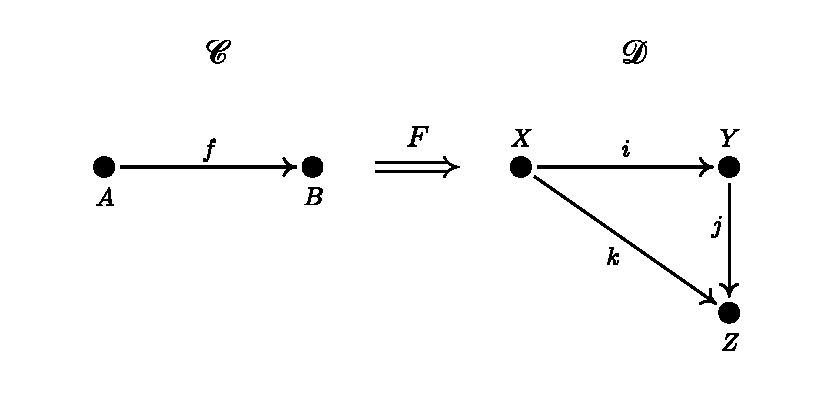
\includegraphics[width=1.1\textwidth]{./notebooks/Functor.pdf}
  \end{center}
  \caption{Diagrams showcasing the properties of Functors.}
  \label{fig:Functor}
\end{figure}

\subsection{Category of Small Categories}

One might realize that functors are acting on categories in a very similar way as morphisms
do to objects. Indeed, we can define a functor composition to be
such that for two functors $F:\mathcal C \Rightarrow \mathcal D$
and $G:\mathcal D \Rightarrow \mathcal E$, then $G \circ F$ is
a functor from $\mathcal C$ to $\mathcal E$ where
\begin{enumerate}
  \item For any $A \in Ob_\mathcal C$, $G\circ F (A) = G(F(A))$,
  \item For any $f \in Mor_\mathcal C$, $G\circ F (f) = G(F(f))$.
\end{enumerate}
We can also define an identity functor $I:\mathcal C \Rightarrow \mathcal C$,
where $F(A) = A$ and $F(f) = f$.

Therefore, we might wonder whether there exists a category of all categories
where objects are categories and morphisms are functors.
The answer is ``no''. Similar to the set of all sets, it can be proven
that this category does not exists. Yet, the category of all \textit{small categories}
does.

Remember, a small category is one where both morphisms and objects are sets.
With this, let's prove our first theorem.
\begin{theorem}[Category of Small Categories]
  Let $Ob_{\textbf{SmCat}}$ be small categories and $Mor_{\textbf{SmCat}}$ be functors.
  This constitutes a category.
\end{theorem}
\begin{proof}
  To prove this, we'll use the fact that in Gödel-Bernays class set theory, the
  axiom \ref{axiom:gb} implies what is called a \textit{comprehension scheme}.
  \begin{proposition}[Comprehension Scheme from \citet{borceux1994handbook}]
    If $\phi(x_1,...,x_n)$ is a formula that the quantification occurs on set variables, then
    there exists a class $A$ such that
    \begin{displaymath}
      (x_1,...,x_n) \in A \iff \phi(x_1,...,x_n).
    \end{displaymath}
  \end{proposition}
  Note that
  \begin{displaymath}
    \mathcal C := \langle Ob_\mathcal C, Mor_\mathcal C \rangle \in \textbf{SmCat} \iff
    \mathcal C \text{ ``is a category''}.
  \end{displaymath}
  Since every $\mathcal C$ is small, then the formula to check whether $\mathcal C$ is a category
  iterates over set variables, i.e. $Ob_\mathcal C$ and $Mor_\mathcal C$.
  Thus, the Comprehension Scheme proposition guarantees that $\textbf{SmCat}$ exists.
\end{proof}

\subsection{Types of Functors}

Before we go on to provide examples of functors, let's present
a way to classify different functors.

\begin{definition}[Faithful, Full, Fully Faithful and Embedding]
  Here we follow \citet{roman2017introduction}.
  Let $F$ be a functor between categories $\mathcal C$ and $\mathcal D$.
  \begin{enumerate}[1.]
    \item $F$ is \textbf{faithful} if for every $A,B \in Ob_\mathcal C$,
      $F:Mor_\mathcal C(A,B)\to Mor_\mathcal C(FA,FB)$ is injective.
    \item $F$ is \textbf{full} if for every $A,B \in Ob_\mathcal C$,
      $F:Mor_\mathcal C(A,B)\to Mor_\mathcal C(FA,FB)$ is surjective.
    \item $F$ is \textbf{fully faithful} if for every $A,B \in Ob_\mathcal C$,
      $F:Mor_\mathcal C(A,B)\to Mor_\mathcal C(FA,FB)$ is bijective.
    \item $F$ is an \textbf{embedding} of $\mathcal C$ in $\mathcal D$ if $F$ is fully faithful
      and $F:Ob_\mathcal C \to Ob_\mathcal D$ is injective.
  \end{enumerate}
 
\end{definition}

\subsection{Subcategories}

\begin{definition}[Subcategory]
  Let $\mathcal D$ be a category. We say that $\mathcal C$
  is a subcategory of $\mathcal D$ if $Ob_\mathcal C \subset Ob_\mathcal D$ and
  $Mor_\mathcal C \subset Mor_\mathcal D$, such that $\mathcal C$ is a category.

  If for every $A, B \in Ob_\mathcal D$, we have that $Mor_\mathcal D (A,B) = Mor_\mathcal C(A,B)$,
  then $\mathcal C$ is a \textit{full subcategory}.
\end{definition}

From the definition of a functor, one might wonder whether for any
functor $F:\mathcal C \Rightarrow \mathcal D$,
the image $F(\mathcal C)$ is a subcategory of $\mathcal D$, i.e.
if $\langle Ob_{F(\mathcal C)}, Mor_{F(\mathcal C)} \rangle$ is a category where
\begin{displaymath}
  Ob_{F(\mathcal C)}:= \{F(A) : A \in Ob_\mathcal C\}, \quad
  Mor_{F(\mathcal C)}:= \{F(f) : f \in Mor_\mathcal C\}.
\end{displaymath}
The answer is no.

\subsection{Relevant Examples of Functors}

Now that we know what a functor is, let's showcase some relevant examples
that might be useful to someone applying Category Theory to another field.

\begin{example}[Power Set Functor]
  The power set functor $\mathcal P : \mathbf{Set} \to \mathbf{Set}$ takes a
  set to it's power set and a function $f:A\to B$ to the image function
  $Im f : \mathcal P(A) \to \mathcal P(B)$, i.e. for a subset $S \subset A$
  in the domain, returns $f(S) := \{ f(x) \ : x \in S\}$.

  Another even more relevant example is the \textit{contravariante} power set
  functor $F : \mathbf{Set} \to \mathbf{Set}$ that takes $A$ to $\mathcal P(A)$
  and $f$ to the inverse image $f^{-1}$.
\end{example}

\begin{example}[Identity Functor]
  This does what one might expect from the name. The identity
  functor is $1_\mathcal C : \mathcal C \to \mathcal C$, such that
  $1_\mathcal C (A) = A \in Ob_\mathcal C$ and
  $1_\mathcal C (f) = f \in Mor_\mathcal C$.
\end{example}

\begin{example}[Inclusion Functor]
  For a subcategory $\mathcal S$ of $\mathcal C$, the inclusion
  functor is $I_\mathcal C : \mathcal S \to \mathcal C$, such that
  $I_\mathcal C (A \in Ob_\mathcal S) = A \in Ob_\mathcal C$ and
  $I_\mathcal C (f \in Mor_\mathcal S) = f \in Mor_\mathcal C$.
\end{example}


\section{Natural Transformations}

Similar to how morphisms define relations between objects in a category, natural transformations
define relations between functors.
The term ``natural'' in natural transformations was coined by Eilenberg and MacLane (the founders
of Category Theory) due to the fact that these transformations were developed with the
aim of explaining why some constructions in Mathematics were ``natural'' while others
were not.


\subsection{Defining Natural Transformations}

Similar to functors, the formal definition of natural transformations
are somewhat obscure at first sight, by as we dig a bit, we see that the is
some intuition behind it that makes it easier to understand it.

\begin{definition}[Natural Transformations]
  Let $\mathcal C$ and $\mathcal D$ be categories, and let $F,G:\mathcal C \to \mathcal D$ be functors.
  A natural transformation $\alpha: F \Rightarrow G$ is such that:
  \begin{enumerate}[(i)]
    \item For all $A \in \mathcal C$, there exists $\alpha_A :F(A) \to G(A)$ that is
      a morphism in $\mathcal D$, i.e $\alpha_A \in Mor_\mathcal D (F(A), G(A))$;
    \item (Naturality) For all $f \in Mor_\mathcal C (A,B)$, then
      \begin{displaymath}
        F(f)\fatsemi \alpha_B = \alpha_A \fatsemi G(f).
      \end{displaymath}

    Remember that for a morphism $f:A \to B$, we have that $F(f):F(A)\to F(B)$ and $G(f):G(A) \to G(B)$.
    Since $\alpha_A: F(A) \to G(A)$ and $\alpha_B : F(B) \to G(B)$, then $F(f)$ composes
    with $\alpha_B$ and $G(f)$ composes with $\alpha_A$, and our definition above works.
  \end{enumerate}
  \label{def:NaturalTransformation}
\end{definition}

Another way to represent property (ii) in the definition of natural transformations
is to affirm that the diagram below.

\begin{figure}[H]
  \begin{center}
    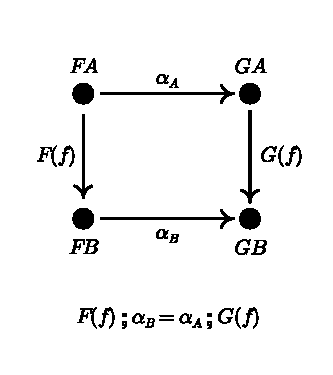
\includegraphics{./notebooks/NaturalTransformation.pdf}
  \end{center}
  \caption{Commutative diagram of a natural transformation highlighting the commutative property of the definition.}
  \label{fig:NaturalTransformation}
\end{figure}

From the definition, the natural transformation $\alpha$ is a transformation between functors
that is in some sense associative, i.e. the order does not matter, we can apply $\alpha$
to $FA$ and then apply $Gf$, or we can apply $Ff$ to $FA$ an then apply the natural transformation. Both
return the same result.

\subsection{The Category of Functors}

The natural transformation is also ideal for defining a category of functors.

\begin{definition}
  For categories $\mathcal C$ and $\mathcal D$, then $\mathcal D^{\mathcal C}$ is the category
  of functors from $\mathcal C$ to $\mathcal D$ where the morphisms are natural transformations,
  i.e.
  \begin{displaymath}
    Ob_{\mathcal D^{\mathcal C}} :={\text{Functors from } \mathcal C \text{ to } \mathcal D}
  \end{displaymath}
  \begin{displaymath}
    Mor_{\mathcal D^{\mathcal C}}(F,G) :={\text{Natural Transformations from } 
    F \text{ to } G}.
  \end{displaymath}
\end{definition}

Let's prove that the definition above is indeed a category.
For that, we need to define a way to compose natural transformations that
is associative, and we also need to define an identity morphism.

\begin{proposition}
  In the category $\mathcal D^{\mathcal C}$, define the composition of two natural
  transformations $\alpha:F\to G$ and $\beta:G\to H$ as
  \begin{displaymath}
    \forall c \in \mathcal C, \ \alpha_c \fatsemi \beta_c = (\alpha \fatsemi \beta)_c.
  \end{displaymath}
  Then, using this definition, $\alpha \fatsemi \beta$ is indeed a normal transformation
  from $F \to H$, and this composition is associative.
\end{proposition}
\begin{proof}
  First, since
  $\alpha_c \in Mor_\mathcal D (F(c),G(c))$,
  $\beta_c \in Mor_\mathcal D (G(c),H(c))$,
  $\gamma_c \in Mor_\mathcal D (H(c),J(c))$,
  then
  \begin{align*}
    \alpha \fatsemi (\beta \fatsemi \gamma) \iff 
    \forall c \in \mathcal C, \alpha_c \fatsemi (\beta \fatsemi \gamma)_c &=
    \alpha_c \fatsemi (\beta_c \fatsemi \gamma_c)\\&=
    (\alpha_c \fatsemi \beta_c) \fatsemi \gamma_c \\&= 
    (\alpha_c \fatsemi \beta_c) \fatsemi \gamma_c \\&= 
    (\alpha \fatsemi \beta)_c \fatsemi \gamma_c
    \iff (\alpha \fatsemi \beta) \fatsemi \gamma.
  \end{align*}
  We proved the associative part. Now, we need to show that such $\alpha \fatsemi \beta$
  is a natural transformation from $F$ to $H$. Take $f:c\to c' \in Mor_\mathcal C$.
  Consider $(\alpha \fatsemi \beta)_{c}:F(c) \to H(c)$, and
  $(\alpha\fatsemi \beta)_{c'}:F(c') \to H(c')$. Note that
  \begin{displaymath}
    F(f) \fatsemi \alpha_{c'} = \alpha_{c} \fatsemi G(f), \quad
    G(f) \fatsemi \beta_{c'} = \beta_{c} \fatsemi H(f).
  \end{displaymath}

  Therefore, we have
  \begin{align*}
    F(f) \fatsemi (\alpha\fatsemi \beta)_{c'} =
    (F(f) \fatsemi \alpha_{c'}) \fatsemi \beta_{c'} &=
    (\alpha_c \fatsemi G(f)) \fatsemi \beta_{c'} \\&=
    \alpha_c \fatsemi (G(f) \fatsemi \beta_{c'}) \\&=
    \alpha_c \fatsemi \beta_c \fatsemi H(f)\\&=
    (\alpha \fatsemi \beta)_c \fatsemi H(f).
  \end{align*}
\end{proof}

Since natural transformations are morphisms between functors in this category of functors,
we can now ponder what would an isomorphism between natural transformations look like.
Remember the definition of a categorical isomorphism \ref{def:CategoricalIsomorphism}.
With such definition, we can prove the following result.

\begin{theorem}[Natural Isomorphism \citep{spivak2014category}]
  Let $\mathcal C$ and $\mathcal D$ be categories, and $F,G:\mathcal C \to \mathcal D$ functors.
  A natural transformation $\alpha : F \to G$ is an isomorphism in $\mathcal D^\mathcal C$
  if and only if $\alpha_c: F(c) \to G(c)$ is an isomorphism in $\mathcal D$ for every
  $c \in Ob_\mathcal C$.
\end{theorem}
\begin{proof}
  Check proposition 5.3.2.12 from \citet{spivak2014category}.
\end{proof}


\begin{example}[Natural Transformations in Sets]
  Consider the categories $\bm 1$ and $\mathbf{Set}$. We wish to
  construct the category $\mathbf{Set}^{\bm 1}$, i.e. of functors from $\bm 1$
  to $\mathbf{Set}$. Since $\bm 1$ has only one object $1$ and one morphisms $id_1$, then each functor
  $F:\bm 1 \to \mathbf{Set}$ is completely defined by $F(1) = S$, where $S$ is a set, and,
  by the definition of a functor, $F(id_1) = id_S$. This means that every functor
  can be indexed by the set to which it takes the object of $\bm 1$, e.g. $F_A$ is the
  functor that $F(1)$ is equal to set $A$.

  Next, we want to define a natural transformation $\alpha: F_A \to F_B$.
  By definition, there are two criteria to satisfy. First,
  for every object $1 \in Ob_{\bm 1}$ we have
  $\alpha_1:F_A(1) \to F_B(1)$ such that $\alpha_1 \in Mor_{\mathbf{Set}}(F_A(1),F_B(1))$.
  Since the only object in $\bm 1$ is $1$, we only need to define $\alpha_1$ to fully define $\alpha$.
  Since $\alpha_1$ must be a morphism of $\mathbf{Set}$, then $\alpha_1$ is a function
  from $A$ to $B$.

  Secondly, for every $f \in Mor_{\bm 1} (1,1)$, it's required that
  \begin{displaymath}
    F_A(f) \fatsemi \alpha_1 = \alpha_1 \fatsemi F_B(f).
  \end{displaymath}
  Again, since the only morphism in $\bm 1$ is $id_1$, we only need to prove that
  \begin{displaymath}
    F_A(id_1) \fatsemi \alpha_1 = \alpha_1 \fatsemi F_B(id_1).
  \end{displaymath}

  Note that $F_A(id_1) = id_A$ and $F_B(id_1) = id_B$, and by the definition
  of the identity, we have that for $g \in Mor(A,B)$, $id_A \fatsemi g = g \fatsemi id_B$.
  Hence, the second condition is trivially satisfied.

  With this, we conclude that the natural transformations from
  functors $F_A$ to $F_B$ are, in a sense, isomorphic to functions from sets
  $A$ to $B$.
  
  Considering the category $\mathbf{SmCat}$ of small categories, we can actually prove
  that $\mathbf{Set}$ and $\mathbf{Set}^{\bm 1}$ are isomorphic.

  Consider the functor
  $I:\mathbf{Set}^{\bm 1} \to \mathbf{Set}$ where $I(F_A) = A \in \mathbf{Set}$ and
  for any natural transformation $\alpha^{(f)}$ where $\alpha^{(f)}_1 = f$, we have
  $I(\alpha^{(f)}) = f$. Also, define $I^{-1}(A) = F_A$ and
  $I^{-1}(f) = \alpha_f$.
  Thus, $I$ defines an isomorphism between the two categories.

\end{example}

\subsection{Equivalence Between Categories}

We've used the existence of two functors $F:\mathcal C \to \mathcal D$ and $G:\mathcal D \to \mathcal C$,
where $F \fatsemi G = id_\mathcal D$ and $G \fatsemi F = id_\mathcal C$,
to define that two categories are equivalent up to an isomorphism.
Note that in the category of small categories, besides morphisms and objects we also
have natural transformations. Thus, we can make use of natural transformations to
define a new notion of equivalence between categories that is less strict then 
the existence of isomorphic functors.

\begin{definition}[Equivalence of Categories]
  We say that a functor $F:\mathcal C \to \mathcal D$ defines an equivalence of
  categories if there exists another functor $G:\mathcal D \to \mathcal C$ and
  two natural transformations
  $\alpha: id_\mathcal C \to G \circ F$ and
  $\beta: id_\mathcal D \to F \circ G$, where $\alpha$ and $\beta$ are natural isomorphisms,
  i.e. for any $c \in \mathcal C$,
  $\alpha_c:id_\mathcal C(c) \to (G \circ F)(c)$ is an
  isomorphism in $\mathcal C$, and for any $d \in \mathcal D$, 
  $\beta_d:id_\mathcal D(d) \to (F \circ G)(d)$ is an isomorphism in $\mathcal D$.

  Moreover, we say that $F$ are $G$ are mutually inverse equivalences.
  \label{def:EquivalenceCategories}
\end{definition}

The above definition is convoluted, so let's try to get some intuition.
First, note that $id_\mathcal C(c) = c \in \mathcal C$, so the natural transformation
$\alpha$ defines for each object $c \in \mathcal C$ a morphism $\alpha_c$ from $c$
to $c' = G(F(c)) \in \mathcal C$, where $c$ and $c'$ are actually isomorphic.

Now it's a bit clearer what is going on. The definition is stating that two
categories are equivalent if there is a pair of functors which are almost the inverse
of one another, but instead of $(F \circ G)(c) = c$ we have that
$(F \circ G )(c) = c'$  where $c'$ is isomorphic to $c$.
Thus, our functors are not inverses, because they scramble the objects, but in the end,
they just exchange objects that are isomorphic to one another, hence, they ``keep everything
almost the same''.

\subsection{Vertical vs Horizontal Compostion}

We already introduced how we compose natural transformations in
a category of functors $\mathcal D^{\mathcal C}$. This composition
is referred by \citet{spivak2014category} as \textit{vertical}, because
it can be depicted by the Figure below.

Yet, there is another type of operation between natural transformations,
called \textit{Whiskering}, also referred as \textit{horizontal composition}
by \citet{spivak2014category}. This time, the name is inspired by
the diagram below.

\begin{definition}[Prewhiskering]
  Let $\mathcal B, \mathcal C, \mathcal D$ be categories, and define
  the following functors $G_1,G_2:\mathcal C \to \mathcal D$,
  $F:\mathcal B \to \mathcal C$ and the natural transformation
  $\alpha: G_1 \to G_2$.
  A \textit{postwhiskering}
  of $\alpha$ by $\mathcal G$ is denoted by $\alpha \diamond G:G_1 \circ F \to G_2 \circ F$,
  where for every $b \in Ob_\mathcal B$, $(\alpha \diamond F)_b:(G_1 \circ F)(b) \to (G_2 \circ F)(b)$
  is defined to be $\alpha_{F(b)}$ 
\end{definition}

\begin{definition}[Postwhiskering]
  Let $\mathcal B, \mathcal C, \mathcal D$ be categories, and define
  the following functors $F_1,F_2:\mathcal B \to \mathcal C$,
  $G:\mathcal C \to \mathcal D$ and the natural transformation
  $\beta F_1 \to F_2$.
  A \textit{postwhiskering}
  of $\beta$ by $\mathcal G$ is denoted by $G \diamond \beta:G \circ F_1 \to G \circ F_2$,
  where for every $c \in Ob_\mathcal C$, $(\beta \diamond G)_b:(G \circ F_1)(c) \to (G \circ F_2)(c)$
  is defined to be $G(\beta_c)$ .
\end{definition}


\begin{definition}[Horizontal Composition/Whiskering of Natural Transformations]
  Let $\mathcal B, \mathcal C, \mathcal D$ be categories, and define
  the following functors $F_1,F_2:\mathcal B \to \mathcal C$,
  $G_1, G_2 :\mathcal C \to \mathcal D$ and the natural transformations
  $\alpha: F_1 \to F_2$, $\beta: G_1 \to G_2$.

  A \textit{postwhiskering}
  of $\alpha$ by $\mathcal F$ is denoted by $\alpha \diamond F:G_1 \circ F_1 \to G_2 \circ F$,
  where for every $b \in Ob_\mathcal B$, $(\alpha \diamond F)_b:G_1 \circ F(b) \to G_2 \circ F(b)$
  is defined to be $\alpha_{F(b)}$ 

  A \textit{prewhiskering}
  of $\beta$ by $\mathcal H$ is denoted by $H \diamond \beta\circ G_1 \to H \circ G_2$,
  where for every $c \in Ob_\mathcal C$, $(H \diamond \beta)_c: H \circ G_1(c) \to H \circ G_2(c)$
  is defined to be $H(\beta_c)$ .

  A \textit{whiskering} (horizontal composition) between two natural transformations
  $\alpha: F_1 \to F_2$ and $\beta:G_1\to G_2$, denoted by
  $\alpha \diamond \beta: $
\end{definition}

\newpage
\section{Limits, Colimits}

Limits and colimits are universal constructions that generalize some of the
categorical concepts we already talked about, such as products,
equalizers, pullbacks and pushouts.
Limits have a terminal sort of universal properties.
Colimits have an initial sort of universal properties.

They are of interest, because whenever a category is complete with
respect to limits or colimits, these end up corresponding to some
classical concept.

\subsection{Cones and Cocones}

Before talking about limits, we need to introduce the notion of a cone and it's dual, the cocone.

\begin{definition}[Cone]
  Let $\mathcal C$ be a \textit{small} category. The (left) cone $\mathcal C^{\lhd}$ is a category constructed
  by adding an object $LC$, called the cone point, into the set of objects of $\mathcal C$,
  and making it an initial object by guaranteeing that there is only one morphism $l_A$ from $LC$ to each
  $A \in Ob_\mathcal C$. In other words, $\mathcal C^{\lhd}$ is a category where:
  \begin{align*}
    Ob(\mathcal C^{\lhd}) &:= \{LC\} \sqcup Ob(\mathcal C),\\
    Mor_{\mathcal C^{\lhd}}(A,B) &:=
    \begin{cases}
      Mor_\mathcal C (A,B)  \quad &\text{if } A,B \in Ob(\mathcal C), \\
      \{l_A\}  \quad &\text{if } A = LC, B \in Ob(\mathcal C), \\
      \{id_{LC}\}  \quad &\text{if } A = LC, B = LC, \\
      \varnothing \quad &\text{if } A \in Ob(\mathcal C), B = LC.
    \end{cases}
  \end{align*}
\end{definition}

As we pointed out, the cocone is just the dual.

\begin{definition}[Cocone (Right Rone)]
  Let $\mathcal C$ be a \textit{small} category. The cocone $\mathcal C^{\rhd}$ is a category constructed
  by adding an object $RC$, called the cone point, into the set of objects of $\mathcal C$,
  and making it an initial object by guaranteeing that there is only one morphism $r_A$ from $A \in Ob_\mathcal C$ to each
  $RC$. In other words, $\mathcal C^{\rhd}$ is a category where:
  \begin{align*}
    Ob(\mathcal C^{\rhd}) &:= \{RC\} \sqcup Ob(\mathcal C),\\
    Mor_{\mathcal C^{\rhd}}(A,B) &:=
    \begin{cases}
      Mor_\mathcal C (A,B)  \quad &\text{if } A,B \in Ob(\mathcal C), \\
      \{r_B\} \quad &\text{if } A = RC, B \in Ob(\mathcal C),\\
      \{id_{RC}\}  \quad &\text{if } A = RC, B = RC, \\
      \varnothing  \quad &\text{if } A = RC, B \in Ob(\mathcal C), \\
    \end{cases}
  \end{align*}
\end{definition}

\textbf{Caution!} When constructing, for example, the cone category, there can
be only a single morphism leaving $LC$. One might be tempted to construct this
category by drawing an arrow from the initial object $LC$ to every object
in the category $\mathcal C$, but this might lead to more than one morphism
from $LC$ to an object.

\begin{example}[Cone in Discrete Categories]
  Let $\mathbf{\underline{3}}$ be the discrete category with three objects.
\end{example}

\begin{example}[Cone in $\mathbf{Gr}$]
  Let $\mathbf{\underline{3}}$ be the discrete category with three objects.
\end{example}


\subsection{Slice Categories}

A slice category is a way to define categories of certain diagrams (functors) inside another category.
The definition by itself is very obscure, so we instead present how to construct the slice
category for \textit{spans} (remember definition \ref{def:Span} and Figure \ref{fig:Span}).
This example makes clear the motivation behind the slice category.

\begin{example}[Category of Spans in $\mathcal C$]

\end{example}

\subsection{Defining Limits and Colimits}


\section{Adjoints}

Adjoints, or, adjunctions, are not easily understood from the definition alone. 
A good reference for a more intuitive description is the blog Math3ma, where the
intuition for adjoints were taken from.


We already saw that when talking about categories, there is a weaker notion
of equivalence \ref{def:EquivalenceCategories}, where instead of
requiring the existence of an isomorphism given by
$F \circ G = id_\mathcal D$ and $F \circ F = id_\mathcal C$, we only
ask for $F \circ G \cong id_\mathcal D$ and $G \circ F \cong id_\mathcal C$.

But can we make this even weaker? This is where adjunctions come in. Instead
of isomorphism, we only ask for the existence of a morphism (which in the
case of functor is a natural transformation) taking
$F\circ G \to id_\mathcal D$ and
$id_\mathcal C \to G\circ F $.



\subsection{General Definitions}

The definition we are going to present assumes that both categories are locally small. This will
be enough for most applications. Yet, there are a more complicated definition that also takes into
account categories that are not locally small. Remember that a category $\mathcal C$
is locally small if for every pair of objects $A$ and $B$, then $Mor_\mathcal C (A,B)$ is a set.
\begin{definition}
  Let $\mathcal C$ and $\mathcal D$ be locally small categories. The adjoints (adjunction) between
  $\mathcal C$ and $\mathcal D$ are the functors
  \begin{displaymath}
    L:\mathcal C \to \mathcal D, \quad R:\mathcal D \to \mathcal C,
  \end{displaymath}
  together with a natural transformation $\alpha$ such that for every
  $A \in \mathcal C$ and $B, \in \mathcal D$,
  \begin{displaymath}
    \alpha_{A,B}: Mor_\mathcal D (L(A), B) \overset{\cong}{\longrightarrow} Mor_\mathcal C (A, R(B)),
  \end{displaymath}
  i.e. for every pair of objects $A \in \mathcal C$  and $B \in \mathcal D$, there is an isomorphism
  between the sets $Mor_\mathcal D(L(A), B)$ and $Mor_\mathcal C (A, R(B))$.
\end{definition}

\begin{shaded}
  \textbf{Adjoints in Category Theory vs. Linear Algebra.} Names are suggestive in Mathematics,
  but even more so in Category Theory. Note that the definition above of an adjoint resembles
  somewhat the idea of adjoint linear transformation in Linear Algebra. Remember:
  \begin{displaymath}
    \langle A x, y \rangle  = \langle x, A^* y \rangle, \quad \forall x,y \in X,
  \end{displaymath}
  where $X$ is our vector space and $A: X \to X$ is a linear transformation.
\end{shaded}

\begin{proposition}
  Let $\mathcal C$ and $\mathcal D$ be two locally small categories, and $F:\mathcal C \to \mathcal D$
  a functor. If both functors $G,G':\mathcal D \to \mathcal C$ are right (or left) adjoints
  to $F$, then there exists a natural isomorphism between $G$ and $G'$.
\end{proposition}
